\documentclass{article}
%\usepackage[utf8]{inputenc}
\usepackage[total={5.5in,9.5in}]{geometry}
\usepackage{fontspec}
\usepackage{unicode-math}
\usepackage{xspace}
\usepackage{graphicx}
%\usepackage{palatino}
\usepackage{textcomp}
\usepackage{amsmath}
\usepackage{makeidx}
\usepackage{hyperref}
\usepackage{xcolor}
\usepackage{listings}
%\usepackage{gitinfo2}

\setmathfont{STIX2Math}[
Extension={.otf},
Path=./STIX2fonts/,
Scale=1]
\setmainfont{STIX2Text}[
Extension={.otf},
Path=./STIX2fonts/,
UprightFont={*-Regular},
BoldFont={*-Bold},
ItalicFont={*-Italic},
BoldItalicFont={*-BoldItalic}]

\hypersetup{colorlinks=true,linkcolor=blue,citecolor=violet}

\newcommand{\map}{\textsc{map}\xspace}
\newcommand{\foi}{\textsc{foi}\xspace}
\newcommand{\eir}{\textsc{eir}\xspace}
\newcommand{\ramp}{\textsc{ramp}\xspace}
\newcommand{\pfpr}{Pf\textsc{pr}\xspace}
\newcommand{\ihme}{\textsc{ihme}\xspace}

\title{Tourist Index in Movement Models}
\author{adolgert@uw.edu}
\date{\today}

\begin{document}

\maketitle

\section{Introduction}
This is about incorporating the tourist index into movement models. Dave sent me an idea, which is copied as Sec.~\ref{sec:davedesk}. There are a couple of equations I added from references, but that's it. We can do a simple calculation of tourist index in Sec.~\ref{sec:calculatetourist}. Then we'll think about how to add it as a covariate to an inference model.

If we start with notation from Daniel's paper~\cite{Citron2021-jt}, then an Eulerian movement model is
\begin{equation}
  \frac{dN_i}{dt} = -\sum_{j=1}^K f_{i,j} N_i + \sum_{j=1}^K f_{j,i} N_j\label{eqn:citron1}
\end{equation}
where $N_i$ are hosts at site $i$, there are $K$ sites, the total number of hosts is constant over time, and $f_{i,j}$ is a rate for hosts at $i$ to travel to $j$. We fix $f_{i,i}=0$ so there is no self-travel. A fully-specified Flux model requires $K(K-1)$ parameters because it's a $K$ by $K$ matrix of fluxes, minus the diagonal.

\section{From the Desk of Dave Smith}\label{sec:davedesk}
If we carved up space into a sensible set of populated patches, we want to form a time spent / time at risk matrix that describes, on average, how much time a person from here spends there.
(I can write this out in much more specific notation, but think about the problem of parameterizing Host movement model for Simple Trip,
\begin{eqnarray}
\frac{dN_{i,i}}{dt}&=&-\sum_{j=1}^K \phi_{i,j}N_{i,i} + \sum_{j=1}^K \tau_{i,j}N_{i,j} \\
\frac{dN_{i,j}}{dt}&=&-\tau_{i,j}N_{i,j}+\phi_{i,j}N_{i,i}\label{eqn:citron2}
\end{eqnarray}
and getting the steady states
\begin{eqnarray}
N_{i,i}^* & = & \frac{1}{1+\sum_{k=1}^K\frac{\phi_{i,k}}{\tau_{i,k}}}N_i \\
N_{i,j}^* & = & \frac{\phi_{i,j}}{\tau_{i,j}} \frac{1}{1+\sum_{k=1}^K\frac{\phi_{i,k}}{\tau_{i,k}}} N_i\label{eqn:citron3}
\end{eqnarray}
from our \textsc{pnas} paper led by Daniel~\cite{Citron2021-jt}.) [In this model, $\phi_{i,j}$ is the rate at which hosts whose home is $i$ travel to $j$ and $\tau_{i,j}$ is the rate of return.]
Let's call the population-normalized steady states of Eq.~\ref{eqn:citron3} the time at risk matrix, $\Psi$. We'll let $N$ be the vector of population densities.
Note that \verb|t(Psi) N| gives me a vector describing the ambient population here.
And lets call \verb|t(Psi) \%*\% N  / N| the tourist index.
It's the ratio of the ambient population to the resident population.
We want to parameterize TaR matrices, so we use some simple rules. Each patch has a size, position, and population density, so we predict who goes where based on (usually) a simple parametric model: e.g. gravity, or radiation.
What if, instead, we started by putting constraints on something like the tourist index, and then we worked back to ask where people came from?
...so the idea for a paper would be to find several published models and compute the tourist index.
ya. I was thinking the one by John Marshall that Sean and Hector were on, for starters~\cite{Marshall2018-wf}.
It's always been hard to formulate travel and check models for gridded population models.
I guess the main idea is really any one of three:
\begin{enumerate}
  \item formulate a model for time at risk that explicitly constrains the tourist index;
  \item formulate models that impose some relationship between covariates and the tourist index and generate time at risk; or 
  \item examine the relationships between the tourist index and covariates in published models.
\end{enumerate}
Before we jumped in feet first, I guess we define a small pilot study and get the lay of the land. The John Marshall\textsuperscript{+} paper is good.


\section{Calculate Some Tourist Indices}\label{sec:calculatetourist}

\subsection{From the Marshall Paper on Mathematical Models}

This paper~\cite{Marshall2018-wf} uses travel data from four countries to evaluate distance kernels for movement. It doesn't use data about the duration of trips and doesn't give trip duration data to readers. For each distance kernel, they fit to find the best parameters, and those parameters are in a table. So this has:
\begin{itemize}
  \item Distance kernels.
  \item Parameter choices for those distance kernels.
  \item Coordinates for population centers and populations at those centers.
\end{itemize}
It's a great paper with great data. What can we do with it?
\begin{enumerate}
  \item Calculate the tourist index for the given kernels, on the given landscapes, with given parameters. This would require adding a length of stay or a distribution of lengths of stay.

  \item Use an estimate of the tourist index to estimation of parameters. Do this by making a prior on the tourist index and including it in the likelihood.
\end{enumerate}
Let's start with the simpler calculation.

\subsection{Relate two travel models}

I don't know the proper term to differentiate a gravity model from a simple trip model. The gravity model is a likelihood for each destination, but it doesn't have a rate of travel. We will see here that we need to add two rates in order to configure a simple trip model from a gravity model.

If we work from a simple trip model, we can consider our core vector to be the total population whose home is each site $i$, $N_i=\sum_j N_{ij}$. Then time time-at-risk matrix is
\begin{equation}
  \psi_{ij}=\frac{N_{ij}}{N_i}.
\end{equation}
This means that all foreigners living at destination $j$ can be written in terms of $\psi$,
\begin{equation}
  \sum_i N_{ij} = \sum_i N_i\psi_{ij}.
\end{equation}
The \emph{tourist index} is that, normalized by the local population.
\begin{equation}
  b_j = \frac{\sum_i N_{ij}}{N_{j}} = \sum_i \frac{N_i\psi_{ij}}{N_{j}}.
\end{equation}
I'm using $b_j$ for the tourist index because $\tau$ is taken, $t$ is always time, and it reminds me of the word \emph{badaud}, which is a silly part of being a tourist. I'm a little unclear on how to normalize the tourist index. We could normalize it by total people at a place, $N_{jj} + \sum_i N_{ij}$. This would give us the right probability if we choose a random person in a place and ask if this is their home. For approximations, we can use $N_j$ or $N_{jj}$, which are people from a place and people from a place who are currently sleeping there.

If we have a distance kernel, $k_{ij}$, then we can relate that to rates, up to a constant of proportionality.
\begin{equation}
  \frac{k_{ij}}{\sum_j k_{ij}} = \frac{\phi_{ij}}{\sum_j \phi_{ij}}
\end{equation}
We can supply that constant if we look up the probability of travel, which the Marshall et al paper discusses at the end of their data section. They use Demographic and Health Surveys (DHS) to estimate how often people travel and stay overnight.

\subsection{Analyze sample data}

Given the data we have, what steps do we need to do?
\begin{enumerate}
  \item Pick a rate at which people travel anywhere (2 trips per year, so 2/365). Pick a rate of return, $\tau_{ij}$. This can be five-day trips, so 1/5.
  \item Calculate $k(i,j)$ for each point in the Excel file by summing over all kernel values and using that as a normalization.
  \item Calculate $N_{ij}$ for each point, and sum it to get total visitors.
\end{enumerate}
The result is in Fig.~\ref{fig:tantour}.

\begin{figure}
\centering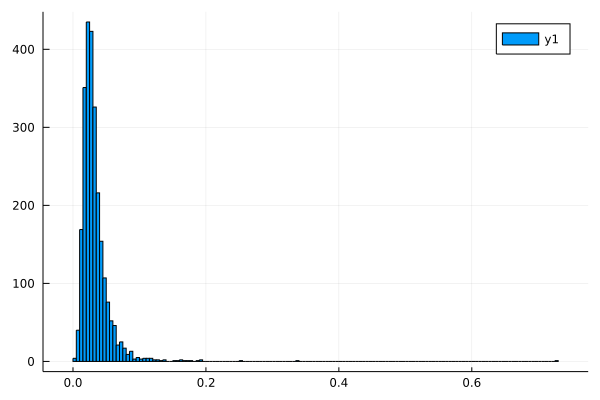
\includegraphics[width=8cm]{tanzania_tourists.png}
\caption{This histogram shows that the tourist index is mostly less than 0.2, with only three outliers, for the Tanzania dataset and parameters from the Marshall paper. It was computed using a repository called \texttt{tourist}.\label{fig:tantour}}
\end{figure}

This quick calculation exercise leads me to observe that, for the simple trip model combined with a gravity model, the ratio of trip frequency to return frequency will determine the time-at-risk matrix. The tourist index would be a one-parameter constraint that ratio. If the simple trip model has $2K(K-1)$ parameters, then we determine them with the $K(K-1)$ parameters given by the gravity model, the $K(K-1) - 1$ parameters from our assertion that $\tau_{i,k}$ is a constant value, and by asserting a value for the single $\sum\phi/\tau$ ratio.

Having calculated the tourist index, and having seen how many parameters it needs, we can think about how to infer a travel model, given the tourist index. That would start with making a likelihood.


\section{Construct a Likelihood}

This section asks how we would infer parameters for a travel model that includes data on the tourist index. This section is incomplete.

\subsection{Destination model likelihood}

This likelihood is simple. Each trip has a choice about where to go. Label trips with $r$.
\begin{equation}
  \prod_{r} \left(\frac{k_{ij}}{\sum_{j} k_{ij}}\right)^{N_r}\label{eqn:destinationlikelihood}
\end{equation}
Let's start with this per-trip probability and write a few things we know, in order to work up to a likelihood that's written in terms of the parameters we want.

\subsection{Simple trip for indistinguishable counts}

We are thinking about a simple trip model. This has a set of interchangeable individuals at sites. Each set of individuals has a home site. When an individual travels to another site, they always return home, not to any other site. There is no interaction among individuals.

The state of the system is the number of individuals at each home site and, for each home site, the number of individuals at each other home site. If the individuals were distinguishable, so we were to talk about one individual, there would be $K^2$ states. Here, there are $K^2$ counts of individuals where each set of $K$ counts adds up to all individuals whose home is one site. These $K^2$ counts are the $N_{ij}$.

In the original problem, without the tourist index, each set of $K$ transitions doesn't interact. Adding a constraint on the tourist index creates an interaction among them. We might be able to write the system as a Kronecker product of simpler systems and then break that symmetry with the tourist constraint.

\subsection{Simple trip for individuals}

Given that there is no interaction among individuals, another way to compute properties of a simple trip is to use individual likelihoods and build up from there.

If we're calculating a single trip with a rate, then the cumulative probability is an exponential distribution.
\begin{equation}
  F(j, t|i) = 1-\frac{k_{ij}}{\sum_jk_{ij}} e^{-\sum_j\lambda_{ij}t}\label{eqn:exponentialsingle}
\end{equation}
Here, the $\lambda_{ij}$ is the rate of trips from $i$ to $j$. It would be $\phi_{ij}$ on the way out and $\tau_{ij}$ on the way back. Note that the exponential factor is the survival until someone leaves the home, also known as the waiting time. If you're thinking about a sequence of these trips, you should be thinking about the Sellke construction.

For a single hop, the likelihood is the pdf of Eq.~\ref{eqn:exponentialsingle}.
\begin{equation}
  f(j, t|i) = \frac{k_{ij}\sum_j\phi_{ij}}{\sum_jk_{ij}} e^{-\sum_j\phi_{ij}t}\label{eqn:pdfsingle}
\end{equation}
If we go out and back with $\phi$ and $\tau$, then each trip has two parts.
\begin{equation}
  f_s(j, t|i) = \frac{k_{ij}\tau_{ij}\sum_j\phi_{ij}}{\sum_jk_{ij}} e^{-\sum_j\phi_{ij}t}e^{-\tau_{ij}t}\label{eqn:pdfsimple}
\end{equation}
If we compute the likelihood of a set of trips, it's the product of these above. All of the time dependence becomes a single term in the log-likelihood, leaving the same calculation as Eq.~\ref{eqn:destinationlikelihood} for the choice of where to travel.

Recall how a single-hop CDF for an exponentially-distributed stochastic process becomes the likelihood of having $m$ jumps in a time $t$. The maximum likelihood of $m$ is $d/dn$ of $\prod f(j,t|i)$. In this case, for the tourist index, you're doing a similar likelihood calculation, but looking at the sum of all transitions into a destination.


\subsection{Disconnect preference from observation}

A simple way to state this problem is to say that there are some place people prefer to go. While each gravity model is independent, the covariate driving the tourist covariate would be shared among gravity models. In this case, we assert a form for the likelihood of travel and calculate its effect on tourist index.

The tourist index would be covariate-driven and could modify the rate for travel to a location.
\begin{equation}
  \lambda = \phi_{ij} + \beta X_{j}
\end{equation}
It might make sense to make it proportional.
\begin{equation}
  \lambda = \phi_{ij}(1 + \beta X_{j})
\end{equation}
We could guarantee it not be negative by using Cox proportional hazards.
\begin{equation}
  \lambda = \phi_{ij}\exp\left(\beta X_{j}\right)
\end{equation}
If we choose one of these forms, what does it do to the tourist index?

The tourist index can be computed from a few similar starting equations. We might have to try different ones to see which works best. Let's start by writing the most intuitive, that it's foreign people in a place, divided by all people in a place. This corresponds to a news report, ``one out of every three people in Santa Monica is from somewhere else.''
\begin{equation}
 b_j = \frac{\sum_{i\ne j} N_{ij}}{\sum_i N_{ij}}\label{eqn:touristexact}
\end{equation}
We know the steady-state $N_{ij}$ from Eq.~\ref{eqn:citron3}. Let's designate $\exp\left(\beta X_{j}\right)$ with $T_j$ and label the new steady state with a prime.
\begin{eqnarray}
N_{i,i}' & = & \frac{1}{1+\sum_{k=1}^K\frac{\phi_{i,k}T_k}{\tau_{i,k}}}N_i \\
N_{i,j}' & = & \frac{\phi_{i,j}T_j}{\tau_{i,j}} N_{i,i}'\label{eqn:touriststable}
\end{eqnarray}
Plug into Eq.~\ref{eqn:touristexact}.
\begin{equation}
b'_j = \frac{\sum_{i\ne j}N_{ij}'}{N'_{jj}+\sum_{i\ne j} N_{ij}'}
\end{equation}
Maybe this simplifies. It isn't obvious to me from here.

We could make the tourist index simplify by requiring that tourist index not change the total rate at which someone leaves a site. This would mean the sum doesn't change.
\begin{equation}
\sum_{k=1}^K\frac{\phi_{i,k}T_k}{\tau_{i,k}} = \sum_{k=1}^K\frac{\phi_{i,k}}{\tau_{i,k}}
\end{equation}
This could be achived by introducing an offsetting constant.
\begin{equation}
  \lambda_{ij} = \phi_{ij}\exp\left(\beta X_{j} + H_i\right)
\end{equation}
It's always possible to find an offsetting constant because we're asking the dot product of two vectors to remain constant, so we're defining a planar subspace, and the constant changes the length of the vector to meet that subspace. This wouldn't quite collapse the equation to be exactly the tourist index, though. I should look at this more.


\section{Pilot}
I propose that we fit to synthetic data, in order to see that a fit can happen. That means I choose a functional form for the destination model and the tourist index, generate from it, and then fit to it. We can do a sequence of progressively more difficult fits.
\begin{enumerate}
  \item The model of one site has no tourist index. Fit that.
  \item The model of one site has a tourist index and data about tourists from that one site.
  \item The model has many sites and tourist index data for each source site, so they are independent. Do this fit in order to see memory requirements.
  \item The model has many sites and tourist index that is a sum of all tourists.
  \end{enumerate}

\subsection{Example of inference}
As an example of the kind of calculation we could do, I made some synthetic data for a travel model and then fit it using probabilistic programming.

This is a gravity model, just that, but I'm not fitting it with a likelihood. I'm fitting it the way we would have to fit the other models, by sampling parameters and simulating an outcome.

In this code, a \verb|TArray| is just an array. The input data is an array, $x$,  of how many trips went to each of $K$ sites. The model is written using a package called Turing.jl.
\begin{lstlisting}
@model function gravity_model(x, ::Type{T} = Float64) where {T <: Real}
    s ~ InverseGamma(2, 3)  # error on observation.
    a ~ Gamma(2, 3)
    r ~ Gamma(2, 0.2)
    k = TArray(T, K)
    for kidx in 1:K
        # The gravity model.
        k[kidx] = Nj[kidx] * (one(T) + distance[kidx] / r)^(-a)
    end
    ktotal = sum(k)

    for dest_idx in 1:K
        x[dest_idx] ~ Normal(1000 * k[dest_idx] / ktotal, 1000 * sqrt(s))
    end
end

chn = sample(gravity_model(trips), HMC(0.1, 5), 1000)
\end{lstlisting}
The fit isn't great with these priors. I need to plot some things, be more careful.

I'm wondering what data we should assume for a travel model that has tourist covariates. That would determine the form of this kind of inference.

\bibliographystyle{ieeetr}
\bibliography{tourist}
\end{document}
